Este capítulo descreve os procedimentos e decisões de projeto adotados no desenvolvimento do sistema integrado de bancada para ensaios de conjuntos motopropulsores. A metodologia está organizada em três frentes de trabalho interdependentes: \textit{Computer-Aided Design} (CAD), a placa de medição e a Interface de Usuário (PC). A placa de medição concentra a aquisição dos sensores da bancada, o acionamento do motor, a segurança e a estimação de rotação e torque a partir das tensões e correntes de fase. Para fins de resultados mais pertinentes à equipe Albatroz Aerodesign, designou-se o motor Scorpion A-5025-310Kv e a bateria LiPo 6S de \SI{3300}{\milli\ampere\hour} 40C, mostrados na \autoref{fig:motor_batata}.

\begin{figure}[H]
    \centering
    \caption{Bateria e Motor}
    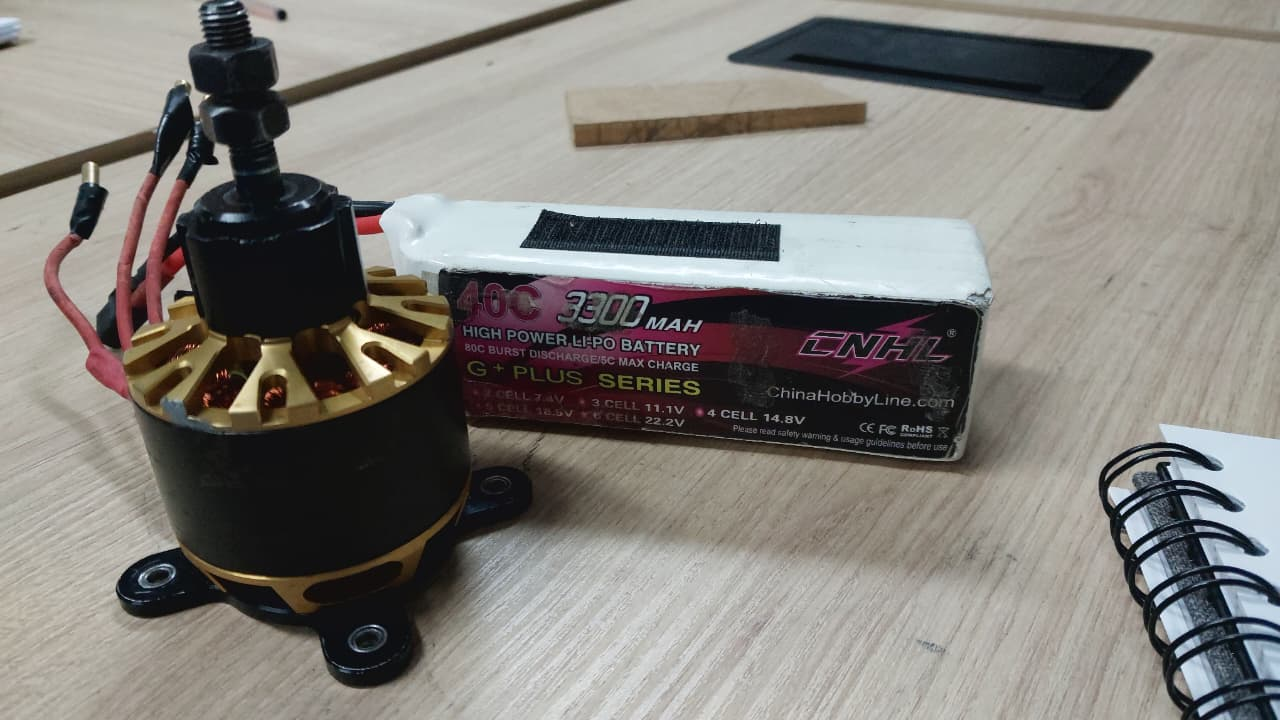
\includegraphics[width=0.5\linewidth]{Textuais/Imgs/Metodologia/Motor_batata.jpeg}
    \label{fig:motor_batata}

    Fonte: Autor (2026)
\end{figure}

A execução metodológica e a sequência lógica deste trabalho são organizadas
em três janelas de transição (Q1, Q2 e Q3), que concentram as
deliberações e decisões mais críticas do desenvolvimento, resumidas na
\autoref{fig:portao_metodologia}: Q1 é a etapa de decisão de projeto, onde
são definidas as restrições e definições de projeto; Q2 é a etapa de
validação individual de cada \textit{feature}; e Q3 é a finalização do
projeto, marcando seu término. As três frentes de trabalho,
\textit{Computer-Aided Design} (CAD), placa de medição e Interface de
Usuário (PC), percorrem essas mesmas três janelas de forma independente,
cada uma com seu próprio fluxo de passos, apresentados nas
\autoref{fig:fluxo_cad} a \autoref{fig:fluxo_interface}.

\begin{figure}[H]
    \centering
    \caption{Janelas de transição da metodologia (Q1, Q2, Q3)}
    \label{fig:portao_metodologia}
    \resizebox{\textwidth}{!}{%
    \begin{tikzpicture}[
        font=\small,
        gate/.style={draw, diamond, aspect=2, align=center, minimum width=2.3cm, minimum height=1.4cm, fill=black!85, text=white, font=\bfseries\small},
        lbl/.style={align=center, text width=3.6cm, font=\small},
        arrow/.style={-{Latex}, thick}
    ]
        \node[gate] (q1) at (0,0)    {Q1};
        \node[gate] (q2) at (5,0)    {Q2};
        \node[gate] (q3) at (10,0)   {Q3};
        \node[gate, fill=black!60] (fim) at (15,0)  {FIM};

        \draw[arrow] (q1) -- (q2);
        \draw[arrow] (q2) -- (q3);
        \draw[arrow] (q3) -- (fim);

        \node[lbl] at (0,-1.6)  {Decisão de projeto:\\restrições e definições};
        \node[lbl] at (5,-1.6)  {Validação individual\\de cada \textit{feature}};
        \node[lbl] at (10,-1.6) {Finalização\\do projeto};
        \node[lbl] at (15,-1.6) {Término\\do TCC};
    \end{tikzpicture}%
    }

    Fonte: Autor (2026)
\end{figure}

\begin{figure}[H]
    \centering
    \caption{Planejamento: CAD}
    \label{fig:fluxo_cad}
    \begin{tikzpicture}[
        font=\small,
        flowbox/.style={draw, rounded corners, fill=white, align=center, minimum width=4.6cm, minimum height=0.9cm, text width=4.3cm},
        halfbox/.style={draw, rounded corners, fill=white, align=center, minimum width=2.9cm, minimum height=1cm, text width=2.6cm},
        arrow/.style={-{Latex}, thick},
        qmark/.style={draw, diamond, fill=black!85, text=white, font=\bfseries\tiny, align=center, minimum width=0.9cm, minimum height=0.6cm, inner sep=0pt}
    ]
        % Faixas de fase (fundo), horizontais
        \fill[green!45!black!25]  (-3.5,2.9) rectangle (3.5,6.9);
        \fill[orange!55!black!20] (-3.5,0.4) rectangle (3.5,2.9);
        \fill[red!55!black!20]    (-3.5,-3)  rectangle (3.5,0.4);

        % Marcadores de transição de fase, na borda esquerda das faixas
        \node[qmark] at (-4.2,6.9) {Q1};
        \draw[-{Triangle[length=2.5mm]}, thick] (-4.2,6.6) -- (-4.2,3.2);
        \node[qmark] at (-4.2,2.9) {Q2};
        \draw[-{Triangle[length=2.5mm]}, thick] (-4.2,2.6) -- (-4.2,0.7);
        \node[qmark] at (-4.2,0.4) {Q3};

        \node[halfbox] (s1) at (-1.9,6.3)  {Diagrama simples\\de alimentação};
        \node[halfbox] (s2) at (1.9,6.3)   {Definição dos\\equipamentos principais};
        \node[flowbox] (s3) at (0,4.6)     {Localização das placas};
        \node[flowbox] (s4) at (0,3.4)     {Definição de restrição\\física das placas};
        \node[flowbox] (s5) at (0,1.6)     {Esboço da bancada física};
        \node[halfbox] (s6) at (-1.9,-0.5) {Montagem das\\placas no gabinete};
        \node[halfbox] (s7) at (1.9,-0.5)  {Modificações\\da bancada};

        \draw[arrow] (s1) -- (s3);
        \draw[arrow] (s2) -- (s3);
        \draw[arrow] (s3) -- (s4);
        \draw[arrow] (s4) -- (s5);
        \draw[arrow] (s5) -- (s6);
        \draw[arrow] (s5) -- (s7);
    \end{tikzpicture}

    Fonte: Autor (2026)
\end{figure}

A frente da placa de medição se desdobra em três trilhas paralelas,
\textit{hardware} (PCB), \textit{firmware} (código) e modelagem do motor e do
observador, lado a lado na \autoref{fig:fluxo_placa}, convergindo para a
validação completa que antecede a integração descrita na \autoref{sec:siba}.

\begin{figure}[H]
    \centering
    \caption{Planejamento: placa de medição}
    \label{fig:fluxo_placa}
    \resizebox{\textwidth}{!}{%
    \begin{tikzpicture}[
        font=\small,
        flowbox/.style={draw, rounded corners, fill=white, align=center, minimum width=4.8cm, minimum height=0.9cm, text width=4.6cm, font=\footnotesize},
        small/.style={draw, rounded corners, fill=white, align=center, minimum width=2cm, minimum height=0.6cm, text width=1.9cm, font=\scriptsize},
        coltitle/.style={align=center, font=\bfseries},
        arrow/.style={-{Latex}, thick},
        qmark/.style={draw, diamond, fill=black!85, text=white, font=\bfseries\tiny, align=center, minimum width=0.9cm, minimum height=0.6cm, inner sep=0pt}
    ]
        % Faixas de fase (fundo), horizontais, cobrindo as três colunas
        \fill[green!45!black!25]  (-8.9,-0.7) rectangle (8.9,5.6);
        \fill[orange!55!black!20] (-8.9,-3.4) rectangle (8.9,-0.7);
        \fill[red!55!black!20]    (-8.9,-7)   rectangle (8.9,-3.4);

        \node[qmark] at (-9.6,5.6)  {Q1};
        \node[qmark] at (-9.6,-0.7) {Q2};
        \node[qmark] at (-9.6,-3.4) {Q3};

        % --- Coluna esquerda: Hardware (PCB) ---
        \node[coltitle] at (-6.0,6) {\textit{Hardware} (PCB)};
        \node[flowbox] (consid) at (-6.0,5.0) {Segurança, alimentação,\\ETH e micro};
        \node[flowbox] (cond)   at (-6.0,3.5) {Condicionamento\\das fases};
        \node[flowbox] (readeq) at (-6.0,2.0) {Readequação\\dos componentes};
        \node[flowbox] (restr)  at (-6.0,0.5) {Restrições físicas};
        \node[small]   (esqpcb) at (-7.15,-1.6) {Esquemático};
        \node[small]   (proto)  at (-4.85,-1.6) {Protótipo};
        \node[flowbox] (valpcb) at (-6.0,-4.5) {Validação das placas};

        \draw[arrow] (consid) -- (cond);
        \draw[arrow] (cond) -- (readeq);
        \draw[arrow] (readeq) -- (restr);
        \draw[arrow] (restr) -- (esqpcb);
        \draw[arrow] (restr) -- (proto);
        \draw[arrow] (esqpcb) -- (valpcb);
        \draw[arrow] (proto) -- (valpcb);
        \draw[-{Latex}, thick, dashed] (valpcb.west) to[bend right=35] node[right, pos=0.5, font=\scriptsize, align=center]{se reprovado,\\refatora} (esqpcb.south west);

        % --- Coluna central: Firmware (Código) ---
        \node[coltitle] at (0,6) {\textit{Firmware} (Código)};
        \node[flowbox] (cod)    at (0,5.1)  {Código};
        \node[flowbox] (dev)    at (0,3.9)  {Compra \textit{dev boards}};
        \node[flowbox] (zephyr) at (0,2.7)  {Criação do projeto em Zephyr};
        \node[flowbox] (amb)    at (0,1.5)  {Criação de ambiente de teste};
        \node[flowbox] (vcore)  at (0,-1.5) {Validação Vcore};
        \node[flowbox] (valsys) at (0,-4.5) {Validação System\\e Application};

        \draw[arrow] (cod) -- (dev);
        \draw[arrow] (dev) -- (zephyr);
        \draw[arrow] (zephyr) -- (amb);
        \draw[arrow] (amb) -- (vcore);
        \draw[arrow] (vcore) -- (valsys);

        % --- Coluna direita: Motor e observador ---
        \node[coltitle] at (6.0,6) {Motor e observador};
        \node[flowbox] (bldc) at (6.0,5.1) {Motor BLDC};
        \node[flowbox] (par)  at (6.0,3.9) {Parâmetros};
        \node[flowbox] (sim)  at (6.0,2.7) {Simulações};
        \node[flowbox] (obs)  at (6.0,1.5) {Observador};
        \node[flowbox] (dbt)  at (6.0,-1.5) {Teste simples\\com \textit{dev board}};
        \node[flowbox] (emb)  at (6.0,-4.5) {Observador embarcado\\na placa};

        \draw[arrow] (bldc) -- (par);
        \draw[arrow] (par) -- (sim);
        \draw[arrow] ([xshift=-6mm]sim.south) -- ([xshift=-6mm]obs.north);
        \draw[arrow] ([xshift=6mm]obs.north) -- ([xshift=6mm]sim.south);
        \draw[arrow] (obs) -- (dbt);
        \draw[arrow] (dbt) -- (emb);

        % Convergência
        \node[flowbox, fill=black!85, text=white] (placa_ok) at (0,-6.3) {Placa de medição completa};
        \draw[arrow] (valpcb.south) |- (placa_ok.west);
        \draw[arrow] (valsys) -- (placa_ok);
        \draw[arrow] (emb.south) |- (placa_ok.east);
    \end{tikzpicture}%
    }

    Fonte: Autor (2026)
\end{figure}

\begin{figure}[H]
    \centering
    \caption{Planejamento: Interface de Usuário (PC)}
    \label{fig:fluxo_interface}
    \begin{tikzpicture}[
        font=\small,
        flowbox/.style={draw, rounded corners, fill=white, align=center, minimum width=4cm, minimum height=0.9cm, text width=3.7cm},
        halfbox/.style={draw, rounded corners, fill=white, align=center, minimum width=2.5cm, minimum height=0.9cm, text width=2.2cm},
        arrow/.style={-{Latex}, thick},
        barrow/.style={{Latex}-{Latex}, thick},
        qmark/.style={draw, diamond, fill=black!85, text=white, font=\bfseries\tiny, align=center, minimum width=0.9cm, minimum height=0.6cm, inner sep=0pt}
    ]
        \fill[green!45!black!25]  (-5.6,2)    rectangle (5.6,5.4);
        \fill[orange!55!black!20] (-5.6,-1.7) rectangle (5.6,2);
        \fill[red!55!black!20]    (-5.6,-6.3) rectangle (5.6,-1.7);

        \node[qmark] at (-6.3,5.4) {Q1};
        \draw[-{Triangle[length=2.5mm]}, thick] (-6.3,5.1) -- (-6.3,2.3);
        \node[qmark] at (-6.3,2) {Q2};
        \draw[-{Triangle[length=2.5mm]}, thick] (-6.3,1.7) -- (-6.3,-1.4);
        \node[qmark] at (-6.3,-1.7) {Q3};

        \node[flowbox] (pc) at (0,4.9)   {PC/\textit{Python}};
        \node[halfbox] (cfg) at (-4.3,3.6) {Arquivos de\\configuração};
        \node[halfbox] (gui) at (4.3,3.6)  {GUI};
        \node[halfbox] (qt)  at (4.3,2.4)  {\textit{Qt Designer}};
        \node[flowbox] (yaml) at (0,2.4)   {Arquivos \textit{yaml}};

        \draw[arrow] (pc) -- (cfg);
        \draw[arrow] (pc) -- (gui);
        \draw[arrow] (gui) -- (qt);
        \draw[arrow] (cfg) -- (yaml);
        \draw[arrow] (gui) -- (yaml);

        \node[flowbox] (tiny) at (0,0.9)  {\textit{TinyTerminal}};
        \node[halfbox] (teste) at (-4.3,0.9) {Teste dos parâmetros\\e comunicação};
        \node[halfbox] (fb) at (4.3,0.9)   {Feedback Membros};

        \draw[arrow] (yaml) -- (tiny);
        \draw[barrow] (tiny) -- (teste);
        \draw[arrow] (tiny) -- (fb);

        % Q3: funcionalidades já implementadas na interface
        \node[flowbox, text width=7.5cm, minimum width=8cm] (feat) at (0,-2.7) {Configuração de sensores, calibração de\\células de carga, \textit{scripts} de estimação\\(SMO, hélice) e registro em CSV};

        \draw[arrow] (teste.south) -- ++(0,-0.7) -| (feat.north);
        \draw[arrow] (fb.south) -- ++(0,-0.7) -| (feat.north);

        \node[flowbox, fill=black!85, text=white] (gui_ok) at (0,-4.6) {Interface Funcional};
        \draw[arrow] (feat) -- (gui_ok);
    \end{tikzpicture}

    Fonte: Autor (2026)
\end{figure}


As três frentes convergem para os testes completos do sistema integrado,
marcando o encerramento da janela Q3 e o término do planejamento do
trabalho.
